
%----------------------------------------------------------------------------------------
% Lecture 5: Phillips Curve + IS-MP Curve (Whelan-style, redrawn in TikZ)
% - Uses output gap notation with unemployment link (Okun) once
% - Figures are original TikZ (inspired by Karl Whelan slides)
%----------------------------------------------------------------------------------------

\documentclass[aspectratio=169,xcolor=dvipsnames]{beamer}
\usetheme{SimpleDarkBlue}

\usepackage{hyperref}
\usepackage{graphicx}
\usepackage{booktabs}
\usepackage{appendixnumberbeamer}
\usepackage{amsmath}
\usepackage{iftex}
\usepackage{tikz}
\usetikzlibrary{arrows.meta,calc}

% --- Font handling (compile anywhere) ---
\ifPDFTeX
  \usepackage[T1]{fontenc}
  \usepackage{lmodern}
  \usepackage{microtype}
\else
  \usepackage{fontspec}
  \usepackage{luatexja}
  \setmainfont{Alegreya Sans Light}[
    ItalicFont={* Italic},
    BoldFont={Alegreya Sans Medium},
    BoldItalicFont={Alegreya Sans Medium Italic}]
  \setsansfont{Alegreya Sans Light}[
    ItalicFont={* Italic},
    BoldFont={Alegreya Sans Medium},
    BoldItalicFont={Alegreya Sans Medium Italic}]
\fi

% ------------------------------------ %
% Section title page with Huge bf text %
% ------------------------------------ %
\AtBeginSection[]{
  \begin{frame}[noframenumbering, plain]
    \Huge{\centerline{\textbf{\insertsection}}}
  \end{frame}
}

%%% automatically add spaces into enumerate and itemize environment
\let\tempone\itemize
\let\temptwo\enditemize
\renewenvironment{itemize}{\tempone\addtolength{\itemsep}{\fill}}{\temptwo}
\let\tempa\enumerate
\let\tempb\endenumerate
\renewenvironment{enumerate}{\tempa\addtolength{\itemsep}{\fill}}{\tempb}

%%=============================================================
%%  FOOTLINE TEMPLATE
%%=============================================================
\defbeamertemplate*{footline}{shadow theme}{%
    \leavevmode\hbox{%
        \hypersetup{linkcolor=white,urlcolor=white,citecolor=white}
        \begin{beamercolorbox}[wd=1.02\paperwidth, ht=2.5ex, dp=1.125ex,
          leftskip=.3cm plus1fil, rightskip=0.3cm]{author in head/foot}%
            \insertsectionnavigationhorizontal{.80\textwidth}{}{} \hspace{.3cm}
            \hfill \#\ \insertframenumber \ / \ \inserttotalframenumber%
        \end{beamercolorbox}%
    }%
}
\setbeamertemplate{footline}[shadow theme]

% --- TikZ styles (clean black lines) ---
\tikzset{
  axis/.style={->,thick},
  curve/.style={thick},
  dsh/.style={thick,dashed},
  >={Latex[length=3mm]},
  lab/.style={fill=white,inner sep=1.3pt,font=\small}
}

% helper: axes with labels
\newcommand{\axes}[4]{% xmin xmax ymin ymax
  \draw[axis] (#1,0) -- (#2,0);
  \draw[axis] (0,#3) -- (0,#4);
}
\newcommand{\xlabel}[1]{\node[below right] at (2.75,0) {#1};}
\newcommand{\ylabel}[1]{\node[above left] at (0,3.95) {#1};}

%----------------------------------------------------------------------------------------
%    TITLE PAGE
%----------------------------------------------------------------------------------------
\title[Phillips Curve]{Macroeconomics II (Spring 2026)\\\vspace{4pt}Lecture 5: Phillips Curve and the IS--MP Curve}
\author[Hui-Jun Chen]{Hui-Jun Chen}
\institute[]{National Tsing Hua University}
\date{}

\begin{document}

%------------------------------------------------
\begin{frame}[plain,noframenumbering]
    \titlepage
\end{frame}

%------------------------------------------------
\section{Why we need a Phillips curve}

%------------------------------------------------
\begin{frame}{From Lecture 3 to a time-series object}
\begin{itemize}
\item AD--AS diagrams: which shocks move $(Y,P)$ together and which move them opposite.
\item To discuss \emph{inflation over time}, we need a relation between:
\begin{itemize}
\item economic slack (output gap) and
\item inflation outcomes.
\end{itemize}
\end{itemize}
\end{frame}

%------------------------------------------------
\begin{frame}{Output gap and unemployment (one connection)}
\begin{itemize}
\item Output gap: $x_t \equiv y_t-y_t^{FE}$.
\item ``Tight labor market'' can be summarized by the unemployment gap:
\[
u_t-u_t^n \approx -\gamma x_t, \qquad \gamma>0.
\]
\item We keep the notation in $x_t$; unemployment is intuition.
\end{itemize}
\end{frame}

%------------------------------------------------
\section{The classic Phillips curve and why it shifts}

%------------------------------------------------
\begin{frame}{The original Phillips curve idea (stylized)}
\begin{columns}
\begin{column}{0.62\textwidth}
\centering
\begin{tikzpicture}[x=1.1cm,y=1.0cm]
  \axes{-2.7}{2.8}{-0.2}{4.0}
  \xlabel{$u_t$ (unemployment)}
  \ylabel{$\pi_t$ (inflation)}

  % downward convex curve
  \draw[curve] (-2.3,3.4) .. controls (-0.8,2.6) and (0.8,1.4) .. (2.3,0.9);
  \node[lab] at (1.6,1.25) {PC};

  % points
  \fill (-1.2,2.8) circle (2pt);
  \fill (1.3,1.35) circle (2pt);
\end{tikzpicture}
\end{column}
\begin{column}{0.38\textwidth}
\small
\begin{itemize}
\item Low unemployment was associated with high inflation.
\item Interpreted as: tight labor markets raise wage growth and price inflation.
\end{itemize}
\end{column}
\end{columns}
\end{frame}

%------------------------------------------------
\begin{frame}{Why this is not stable: expectations}
\begin{itemize}
\item If workers and firms expect higher inflation, wage/price setting adjusts.
\item A stable ``tradeoff'' disappears once expected inflation drifts up.
\item So the curve must include expected inflation as a determinant of actual inflation.
\end{itemize}
\end{frame}

%------------------------------------------------
\begin{frame}{Expectations-augmented Phillips curve (math)}
\small
We will use the same form as Whelan:
\[
\pi_t = \pi_t^{e} + \gamma \big(y_t-y_t^{\ast}\big) + \varepsilon_t^{\pi}.
\]
\begin{itemize}
\item $\pi_t^e$: expected inflation (built into wage/price setting).
\item $y_t-y_t^\ast$ is the output gap (we will also write it as $x_t$).
\item $\varepsilon_t^\pi$: inflationary (cost-push / supply) shock.
\end{itemize}

\vspace{0.3em}
\[
\text{Equivalently:}\quad \pi_t = \pi_t^{e} + \gamma x_t + \varepsilon_t^{\pi}.
\]
\end{frame}

%------------------------------------------------
\begin{frame}{Phillips curve in $(y,\pi)$ space when $\varepsilon_t^\pi=0$}
\begin{columns}
\begin{column}{0.62\textwidth}
\centering
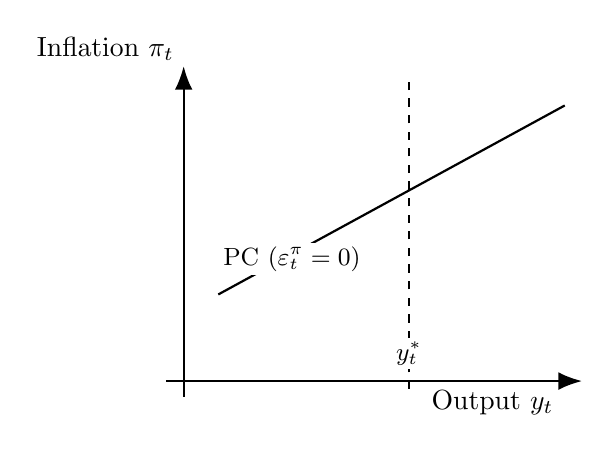
\begin{tikzpicture}[x=1.1cm,y=1.0cm]
  \axes{-0.2}{4.6}{-0.2}{4.0}
  \xlabel{Output $y_t$}
  \ylabel{Inflation $\pi_t$}

  % natural output vertical
  \draw[dsh] (2.6,-0.1) -- (2.6,3.9);
  \node[lab] at (2.6,0.35) {$y_t^\ast$};

  % PC line (upward)
  \draw[curve] (0.4,1.1) -- (4.4,3.5);
  \node[lab] at (1.25,1.55) {PC ($\varepsilon_t^\pi=0$)};
\end{tikzpicture}
\end{column}
\begin{column}{0.38\textwidth}
\small
\begin{itemize}
\item For a given $\pi_t^e$, higher output relative to $y^\ast$ implies higher inflation.
\item $y^\ast$ is potential output (consistent with natural unemployment).
\end{itemize}
\end{column}
\end{columns}
\end{frame}

%------------------------------------------------
\begin{frame}{A supply (cost-push) shock shifts the Phillips curve up}
\begin{columns}
\begin{column}{0.62\textwidth}
\centering
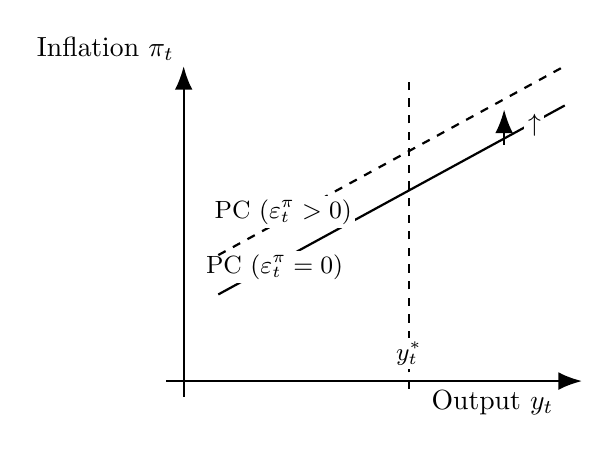
\begin{tikzpicture}[x=1.1cm,y=1.0cm]
  \axes{-0.2}{4.6}{-0.2}{4.0}
  \xlabel{Output $y_t$}
  \ylabel{Inflation $\pi_t$}

  \draw[dsh] (2.6,-0.1) -- (2.6,3.9);
  \node[lab] at (2.6,0.35) {$y_t^\ast$};

  % PC baseline
  \draw[curve] (0.4,1.1) -- (4.4,3.5);
  \node[lab] at (1.05,1.45) {PC ($\varepsilon_t^\pi=0$)};

  % shifted up PC
  \draw[dsh] (0.4,1.6) -- (4.4,4.0);
  \node[lab] at (1.15,2.15) {PC ($\varepsilon_t^\pi>0$)};

  \draw[->,thick] (3.7,3.0) -- (3.7,3.45);
  \node[lab] at (4.05,3.25) {$\uparrow$};
\end{tikzpicture}
\end{column}
\begin{column}{0.38\textwidth}
\small
\begin{itemize}
\item $\varepsilon_t^\pi>0$ raises inflation for any given $y_t$.
\item This is the equation version of ``AS shifts up/left'' in Lecture 3.
\end{itemize}
\end{column}
\end{columns}
\end{frame}

%------------------------------------------------
\begin{frame}{Higher expected inflation shifts the Phillips curve up}
\begin{columns}
\begin{column}{0.62\textwidth}
\centering
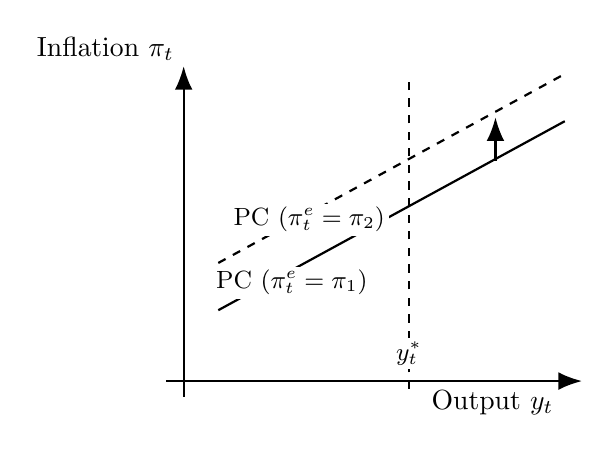
\begin{tikzpicture}[x=1.1cm,y=1.0cm]
  \axes{-0.2}{4.6}{-0.2}{4.0}
  \xlabel{Output $y_t$}
  \ylabel{Inflation $\pi_t$}

  \draw[dsh] (2.6,-0.1) -- (2.6,3.9);
  \node[lab] at (2.6,0.35) {$y_t^\ast$};

  % PC low exp
  \draw[curve] (0.4,0.9) -- (4.4,3.3);
  \node[lab] at (1.25,1.25) {PC ($\pi_t^e=\pi_1$)};

  % PC high exp
  \draw[dsh] (0.4,1.5) -- (4.4,3.9);
  \node[lab] at (1.45,2.05) {PC ($\pi_t^e=\pi_2$)};

  \draw[->,thick] (3.6,2.8) -- (3.6,3.35);
\end{tikzpicture}
\end{column}
\begin{column}{0.38\textwidth}
\small
\begin{itemize}
\item If expectations drift up, inflation stays high even without overheating.
\item ``Anchoring expectations'' means preventing persistent upward shifts.
\end{itemize}
\end{column}
\end{columns}
\end{frame}

%------------------------------------------------
\section{IS curve: output depends on real interest rates}

%------------------------------------------------
\begin{frame}{Real vs nominal interest rates (why Fisher matters)}
\begin{itemize}
\item Nominal rate $i_t$ is the quoted rate.
\item Real rate adjusts for inflation:
\[
r_t \approx i_t-\pi_t.
\]
\item Spending decisions depend on real interest rates (cost of borrowing / reward to saving).
\end{itemize}
\end{frame}

%------------------------------------------------
\begin{frame}{Whelan's IS curve (math)}
\small
Whelan writes:
\[
y_t = y_t^\ast - \alpha \big(i_t-\pi_t-r^\ast\big) + \varepsilon_t^y.
\]
\begin{itemize}
\item $i_t-\pi_t$ is the real interest rate.
\item $r^\ast$ is the natural real rate (consistent with $y_t=y_t^\ast$ on average).
\item $\varepsilon_t^y$ is a demand shock shifting the IS relationship.
\end{itemize}

\vspace{0.3em}
Equivalently in gap form:
\[
x_t = -\alpha\big((i_t-\pi_t)-r^\ast\big)+\varepsilon_t^y.
\]
\end{frame}

%------------------------------------------------
\begin{frame}{IS curve in $(y,r)$ space (picture)}
\begin{columns}
\begin{column}{0.62\textwidth}
\centering
\begin{tikzpicture}[x=1.1cm,y=1.0cm]
  % axes: output on x, real rate on y
  \draw[axis] (-0.2,0) -- (4.7,0) node[below right] {Output $y_t$};
  \draw[axis] (0,-0.2) -- (0,4.0) node[above left] {Real rate $r_t$};

  % downward IS in (y,r): r = a - b y
  \draw[curve] (0.5,3.4) -- (4.4,1.0);
  \node[lab] at (1.3,3.0) {IS};

  \draw[dsh] (2.6,-0.1) -- (2.6,3.9);
  \node[lab] at (2.6,0.35) {$y_t^\ast$};

  \draw[dsh] (-0.1,2.2) -- (4.6,2.2);
  \node[lab] at (0.7,2.35) {$r^\ast$};
\end{tikzpicture}
\end{column}
\begin{column}{0.38\textwidth}
\small
\begin{itemize}
\item Higher real rates reduce demand $\Rightarrow$ lower output.
\item Demand shocks shift IS (move the curve).
\end{itemize}
\end{column}
\end{columns}
\end{frame}

%------------------------------------------------
\section{Monetary policy rule and the IS--MP curve}

%------------------------------------------------
\begin{frame}{A simple inflation-targeting rule (Whelan's MP rule)}
\small
Whelan starts with:
\[
i_t = r^\ast + \pi^\ast + \beta_\pi(\pi_t-\pi^\ast),
\qquad \beta_\pi>0.
\]
\begin{itemize}
\item If inflation rises above target, the bank raises the nominal rate.
\item When $\pi_t=\pi^\ast$, the real rate equals $r^\ast$.
\end{itemize}
\end{frame}

%------------------------------------------------
\begin{frame}{Derive the IS--MP curve: substitute MP into IS}
\small
Start from the IS gap form:
\[
x_t = -\alpha\big((i_t-\pi_t)-r^\ast\big)+\varepsilon_t^y.
\]
Substitute $i_t = r^\ast+\pi^\ast+\beta_\pi(\pi_t-\pi^\ast)$:
\[
i_t-\pi_t-r^\ast = \pi^\ast + \beta_\pi(\pi_t-\pi^\ast) - \pi_t
= (\beta_\pi-1)(\pi_t-\pi^\ast).
\]
Therefore:
\[
x_t = -\alpha(\beta_\pi-1)(\pi_t-\pi^\ast) + \varepsilon_t^y.
\]
\begin{itemize}
\item When $\beta_\pi>1$, IS--MP slopes down in $(x,\pi)$ space.
\end{itemize}
\end{frame}

%------------------------------------------------
\begin{frame}{IS--MP in $(y,\pi)$ space (picture)}
\begin{columns}
\begin{column}{0.62\textwidth}
\centering
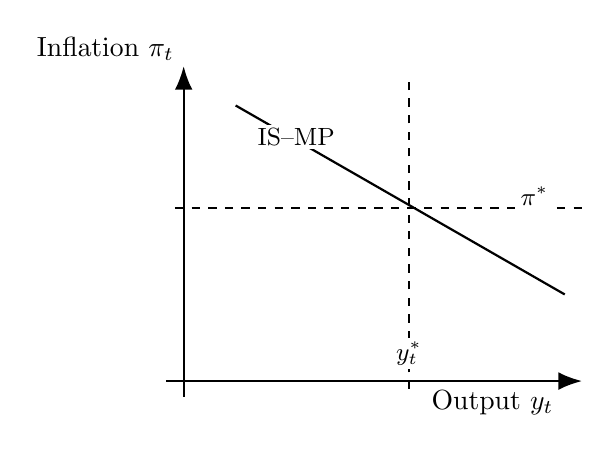
\begin{tikzpicture}[x=1.1cm,y=1.0cm]
  \axes{-0.2}{4.6}{-0.2}{4.0}
  \xlabel{Output $y_t$}
  \ylabel{Inflation $\pi_t$}

  \draw[dsh] (2.6,-0.1) -- (2.6,3.9);
  \node[lab] at (2.6,0.35) {$y_t^\ast$};

  \draw[dsh] (-0.1,2.2) -- (4.6,2.2);
  \node[lab] at (4.05,2.35) {$\pi^\ast$};

  % IS-MP downward in (y,pi)
  \draw[curve] (0.6,3.5) -- (4.4,1.1);
  \node[lab] at (1.3,3.1) {IS--MP};

\end{tikzpicture}
\end{column}
\begin{column}{0.38\textwidth}
\small
\begin{itemize}
\item Higher inflation triggers higher $i_t$.
\item With $\beta_\pi>1$, the real rate rises and output falls.
\end{itemize}
\end{column}
\end{columns}
\end{frame}

%------------------------------------------------
\begin{frame}{Equilibrium: IS--MP + Phillips curve}
\begin{columns}
\begin{column}{0.62\textwidth}
\centering
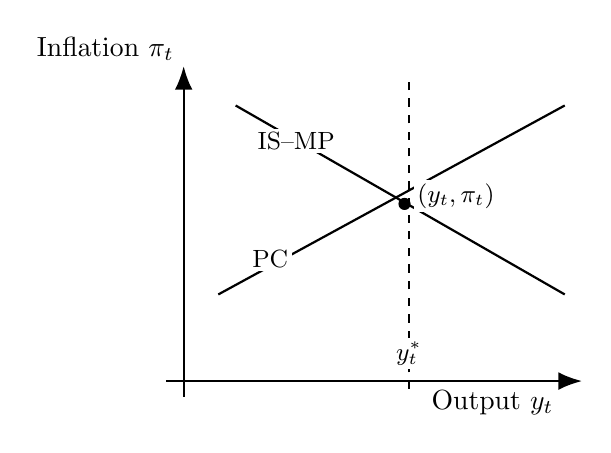
\begin{tikzpicture}[x=1.1cm,y=1.0cm]
  \axes{-0.2}{4.6}{-0.2}{4.0}
  \xlabel{Output $y_t$}
  \ylabel{Inflation $\pi_t$}

  \draw[dsh] (2.6,-0.1) -- (2.6,3.9);
  \node[lab] at (2.6,0.35) {$y_t^\ast$};

  % Phillips curve (upward)
  \draw[curve] (0.4,1.1) -- (4.4,3.5);
  \node[lab] at (1.0,1.55) {PC};

  % IS-MP downward
  \draw[curve] (0.6,3.5) -- (4.4,1.1);
  \node[lab] at (1.3,3.05) {IS--MP};

  % intersection
  \coordinate (E) at (2.55,2.25);
  \fill (E) circle (2.2pt);
  \node[lab,anchor=west] at ($(E)+(0.10,0.10)$) {$(y_t,\pi_t)$};
\end{tikzpicture}
\end{column}
\begin{column}{0.38\textwidth}
\small
\begin{itemize}
\item PC tells how inflation responds to the output gap and expectations.
\item IS--MP tells how output responds to inflation via policy.
\item Intersection determines output and inflation (one-period outcome).
\end{itemize}
\end{column}
\end{columns}
\end{frame}

%------------------------------------------------
\begin{frame}{A more complete Taylor rule (preview)}
\small
Whelan also considers:
\[
i_t = r^\ast+\pi^\ast+\beta_\pi(\pi_t-\pi^\ast)+\beta_y(y_t-y_t^\ast).
\]
\begin{itemize}
\item Responding to the output gap changes the slope of IS--MP, but not the basic logic.
\item This matches your Lecture 4 notation where $i_t$ responds to both $(\pi_t-\pi^\ast)$ and $x_t$.
\end{itemize}
\end{frame}

%------------------------------------------------
\section{Reading this relative to your Lecture 4}

%------------------------------------------------
\begin{frame}{Is Whelan's IS and MP the same as our Lecture 4 notation?}
\begin{itemize}
\item Yes---up to notation choices.
\item Your Lecture 4 gap-IS: $x_t=-\sigma(r_t-r_t^n)+\varepsilon_t^d$.
\item Whelan's IS: $x_t=-\alpha((i_t-\pi_t)-r^\ast)+\varepsilon_t^y$.
\end{itemize}

\begin{itemize}
\item Your Lecture 4 MP rule: $i_t=\bar i+\phi_\pi(\pi_t-\pi^\ast)+\phi_x x_t$.
\item Whelan's baseline MP: $i_t=r^\ast+\pi^\ast+\beta_\pi(\pi_t-\pi^\ast)$ is the special case $\phi_x=0$ and intercept $r^\ast+\pi^\ast$.
\item His ``more complicated rule'' adds $\beta_y(y_t-y_t^\ast)$, matching your $\phi_x x_t$ term.
\end{itemize}
\end{frame}

%------------------------------------------------
\begin{frame}{Next time}
\begin{itemize}
\item Specify a rule for expected inflation $\pi_t^e$ (anchored vs adaptive vs forward-looking).
\item Then we can turn the one-period system into a dynamic inflation model.
\end{itemize}
\end{frame}

\end{document}
